\section{Preprocessing and Feature Engineering}
\label{sec:features}

\subsection{Tier 1: Preprocessing}
Raw eye-tracking recordings contain blinks, boundary violations, and micro-saccade oscillations. We apply two sequential filters. \textbf{(1) Spatial filter:} fixations outside the $1024{\times}768$ stimulus screen are discarded ($5{,}037$ of $293{,}740$ raw fixations removed; $1.71\%$). \textbf{(2) Temporal filter:} fixations shorter than 50\,ms are removed as post-saccadic tremor artifacts ($7{,}666$ removed; $2.66\%$), \rev{yielding $281{,}037$ clean fixations across 16,716 total trials. This results in an average of $16.81 \pm 7.73$ fixations per subject per stimulus image (median: 15, max: 44, with $75\%$ of trials containing 20 or fewer fixations), while preserving the pupil size metrics (\texttt{FIX\_PUPIL}). Fig.~\ref{fig:tier1_filtering} visualizes these filtering steps on a sample scanpath.}

\begin{figure}[htbp]
\centering
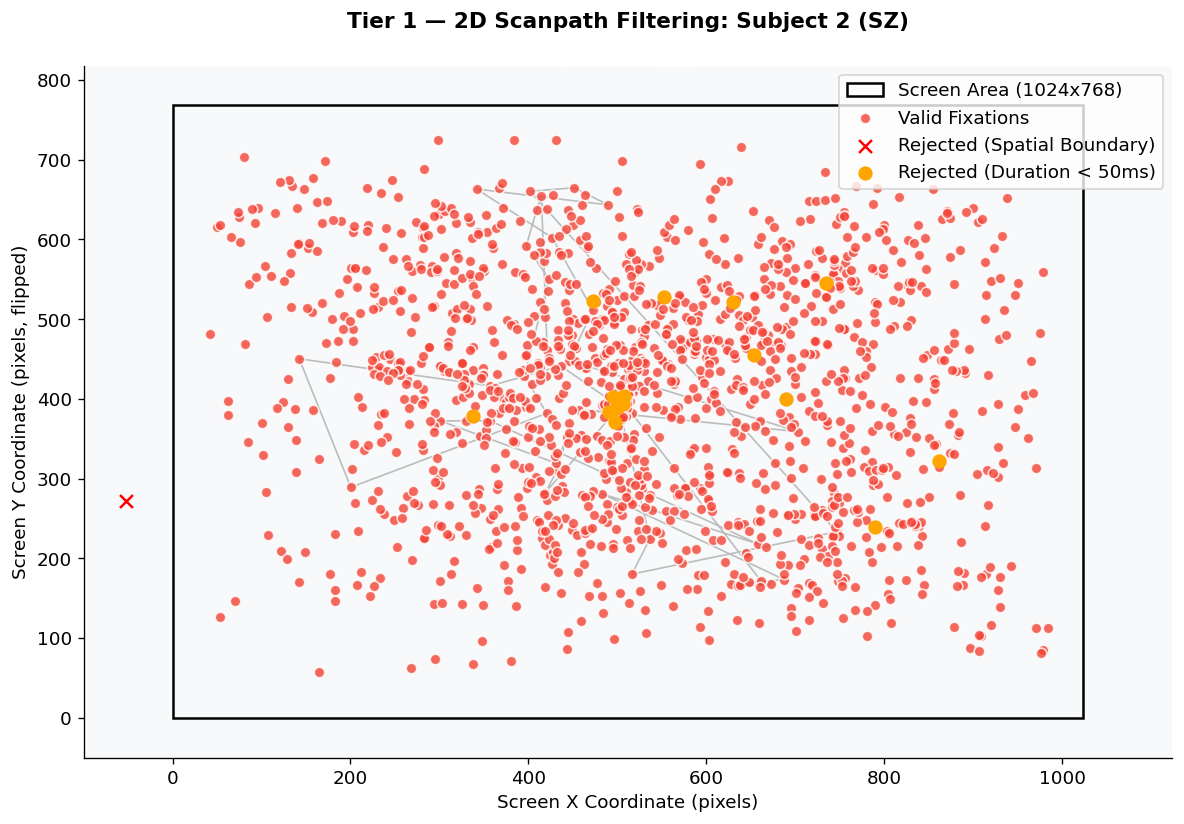
\includegraphics[width=0.95\columnwidth]{tier1_2d_filtering.png}
\vspace{-2mm}
\caption{\rev{Tier 1 scanpath preprocessing visualization for a sample subject. The black rectangle defines the stimulus screen boundaries ($1024\times768$). Red circles represent valid fixations, while red crosses represent fixations rejected due to boundary violations (spatial filtering), and orange circles indicate fixations shorter than 50\,ms rejected as post-saccadic tremor artifacts (temporal filtering).}}
\vspace{-3mm}
\label{fig:tier1_filtering}
\end{figure}

\begin{figure*}[t]
\centering
\resizebox{\textwidth}{!}{%
\begin{tikzpicture}[
    tier/.style={rectangle, draw=blue!70!black, fill=blue!5, rounded corners=4pt,
                 text width=11.5em, text centered, minimum height=4.2em, font=\small\bfseries},
    arrow/.style={->, >=stealth, thick, black!70},
    line/.style={draw, thick, black!70}
]

% Dashed Stream Boxes (drawn in background)
\draw[dashed, orange!80!black, fill=orange!3, rounded corners=4pt] (1.0, 0.6) rectangle (5.0, 2.4);
\node[text=orange!80!black, font=\small\bfseries] at (3.0, 2.6) {Tabular Stream};

\draw[dashed, green!60!black, fill=green!3, rounded corners=4pt] (1.0, -3.4) rectangle (5.0, 0.4);
\node[text=green!60!black, font=\small\bfseries] at (3.0, -3.6) {Deep Sequential Stream};

% Nodes definition
\node[tier] (t1) at (-7.5, -0.5) {Tier 1: Preprocessing\\(Spatial \& Temporal Filtering)};
\node[tier] (t2) at (-2.5, -0.5) {Tier 2: Feature Engineering\\(15 Gaze + 120 Delta Feats)};

\node[tier] (t3) at (3.0, 1.5) {Tier 3: Tabular Baselines\\(CatBoost / XGBoost / LGBM)};
\node[tier] (t4a) at (3.0, -0.5) {Tier 4A: GNN-CEFAM\\(Scanpath Graph + ResNet50)};
\node[tier] (t4b) at (3.0, -2.5) {Tier 4B: BiCA-HS\\(Scanpath Seq + Transformer)};

\node[tier] (t5) at (8.8, -0.5) {Tier 5: OOF Meta-Learner\\(L2-Logistic Regression)};

\node[circle, draw=red!60!black, fill=red!10, inner sep=3pt, font=\small\bfseries] (out) at (12.3, -0.5) {P(SZ)};

% Connections
\draw[arrow] (-11.5, -0.5) node[left, font=\small\bfseries] {Raw Gaze Data} -- (t1);
\draw[arrow] (t1) -- (t2);

% Split to streams
\draw[line] (t2.east) -- ($(t2.east) + (0.5, 0)$);
\draw[arrow] ($(t2.east) + (0.5, 0)$) |- (t3.west);
\draw[arrow] ($(t2.east) + (0.5, 0)$) |- (t4a.west);
\draw[arrow] ($(t2.east) + (0.5, 0)$) |- (t4b.west);

% Merge to meta-learner
\draw[line] (t3.east) -| ($(t5.west) - (0.5, 0)$);
\draw[line] (t4a.east) -- ($(t5.west) - (0.5, 0)$);
\draw[line] (t4b.east) -| ($(t5.west) - (0.5, 0)$);
\draw[arrow] ($(t5.west) - (0.5, 0)$) -- (t5.west);

\draw[arrow] (t5.east) -- (out);

\end{tikzpicture}
}
\caption{\rev{Overview of the proposed Hierarchical 5-Tier Framework. Gaze data is preprocessed (Tier 1) and transformed into stimulus-level and subject-level features (Tier 2). These features feed tabular baselines (Tier 3) and deep architectures (Tier 4) in parallel. The resulting predictions are ensembled by an out-of-fold logistic regression meta-learner (Tier 5) to output the final probability of schizophrenia, $P(\text{SZ})$.}}
\label{fig:pipeline_overview}
\end{figure*}

\subsection{Tier 2: Feature Engineering}

\subsubsection{Tier 2A: Stimulus-Level Features}
For each subject$\times$stimulus trial we extract 15 features spanning four gaze domains:
\begin{itemize}[noitemsep,topsep=2pt]
    \item \textbf{Fixation statistics:} count, mean/median/std of duration.
    \item \textbf{Saccade dynamics:} amplitude mean/std; SA-FDR ($\text{SA-FDR}_i{=}\text{Amp}_i/\text{Dur}_{i+1}$, serving as a visual exploration ratio and cognitive speed proxy); mean turning angle.
    \item \textbf{Scanpath geometry:} total length; \rev{center bias (defined as the mean Euclidean distance of all fixations in a trial from the screen center $(X_c, Y_c) = (W/2, H/2)$ where $W, H$ are the stimulus screen width and height; a smaller average distance indicates a higher tendency to focus on the center);} convex hull area; 2-D spatial entropy ($10{\times}10$ grid).
    \item \textbf{Pupil dynamics:} mean, std, coefficient of variation (CV).
\end{itemize}

\subsubsection{Tier 2B: Contextual Delta Features}
\rev{SZ patients show stimulus-specific visual avoidance, particularly for social and complex scenes. The 100 EMS stimuli belong to four categories: Social (Soc), Natural (Nat), Synthetic (Syn), Manipulated (Man).}

\rev{Specifically, for a subject and a gaze feature $f$, the category mean is defined as:}
\begin{equation}
    \rev{\mu_{c}(f) = \frac{1}{|I_c|} \sum_{i \in I_c} f(i)}
\end{equation}
\rev{where $I_c$ represents the set of trials of category $c \in \{\text{Soc}, \text{Nat}, \text{Syn}, \text{Man}\}$.}

\rev{To capture context-dependent visual responses, we compute pairwise delta features representing the difference in mean responses between categories:}
\begin{equation}
    \rev{\Delta_{c_1 - c_2}(f) = \mu_{c_1}(f) - \mu_{c_2}(f)}
\end{equation}
\rev{for the four diagnostic pairs: (Soc, Nat), (Man, Nat), (Soc, Syn), and (Man, Syn). This yields $15 \text{ features} \times 4 \text{ category-means} = 60$ features, and $15 \text{ features} \times 4 \text{ delta-pairs} = 60$ features, totaling 120 subject-level features. These 120 subject-level features are broadcast to all trials of the subject and concatenated with the 15 trial-specific stimulus-level features, yielding the \textbf{135-dim expert vector} $\mathbf{x}_\text{exp}$ used by Tier~3 and the expert streams of Tier~4.}

SHAP analysis (Fig.~\ref{fig:feature_analysis}, right) confirms that delta features — especially $\Delta_\text{Soc-Nat}$ fixation count and center bias — are the top CatBoost predictors, validating the clinical motivation for Tier~2B. The Pearson correlation matrix (Fig.~\ref{fig:feature_analysis}, left) shows that spatial and saccade features are moderately correlated ($|r|{<}0.6$), confirming near-orthogonal diagnostic contributions.

\begin{figure}[htbp]
\centering
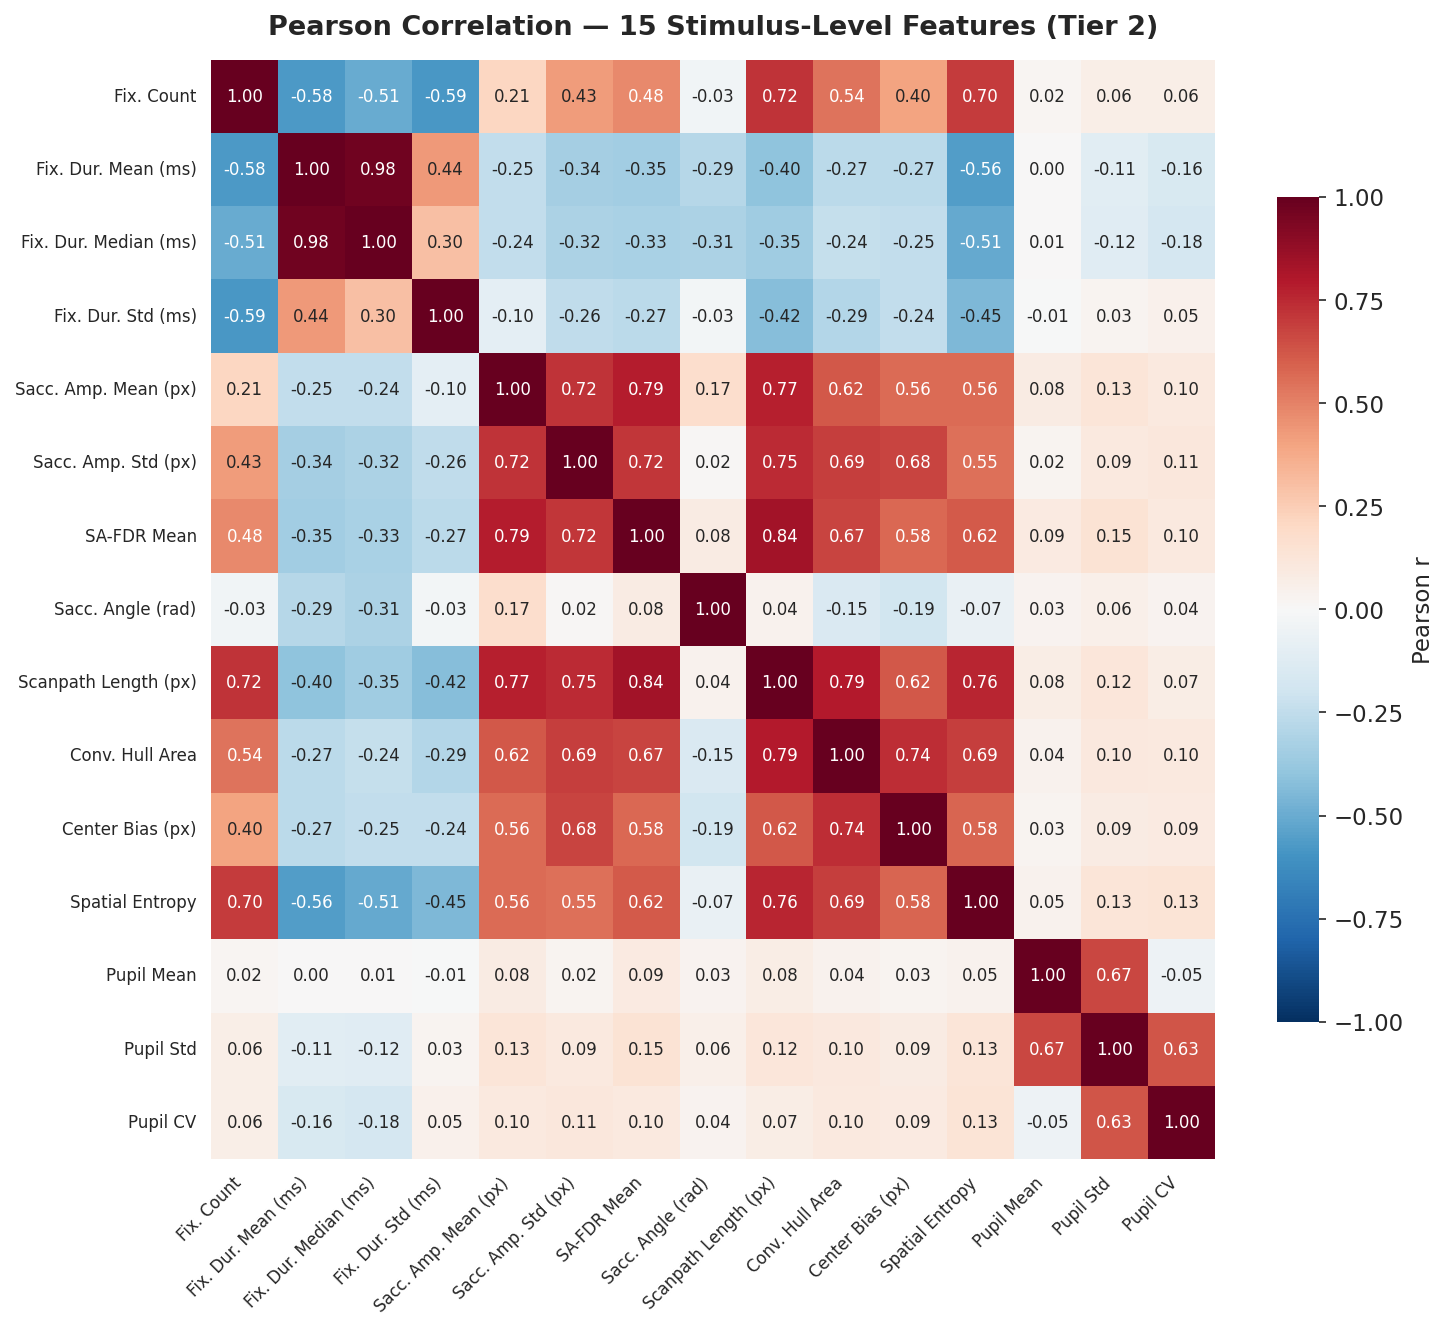
\includegraphics[width=0.48\columnwidth]{tier2_correlation_heatmap.png}\hfill
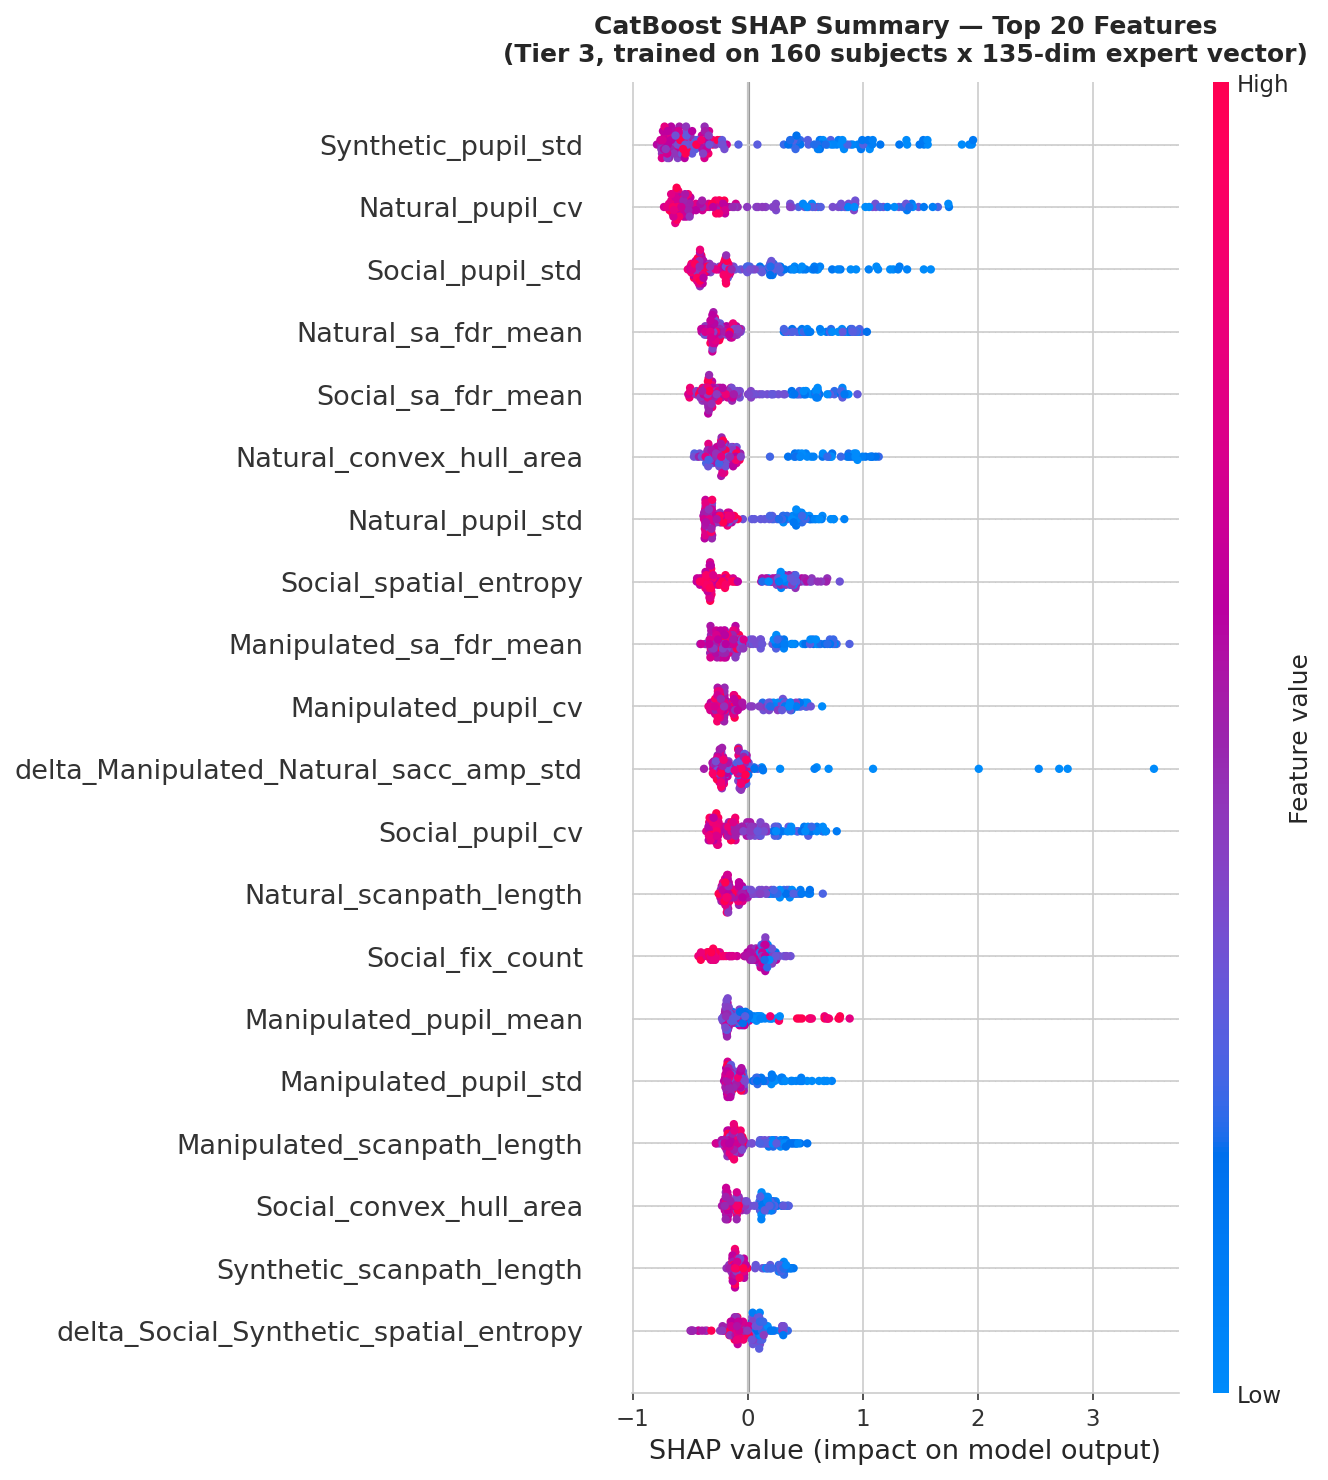
\includegraphics[width=0.48\columnwidth]{tier3_shap_summary.png}
\vspace{-2mm}
\caption{(Left) Pearson correlation of the 15 stimulus-level features. (Right) CatBoost SHAP beeswarm — top 20 features by mean $|\text{SHAP}|$. Delta features $\Delta_\text{Soc-Nat}$ dominate, confirming the clinical value of Tier~2B.}
\vspace{-3mm}
\label{fig:feature_analysis}
\end{figure}

\begin{figure*}[t]
\centering
\resizebox{\textwidth}{!}{%
\begin{tikzpicture}[
    bk/.style={rectangle, draw=blue!60!black, fill=blue!7, rounded corners=3pt,
               text width=10.5em, text centered, minimum height=2.4em, font=\small},
    ek/.style={rectangle, draw=orange!70!black, fill=orange!9, rounded corners=3pt,
               text width=10.5em, text centered, minimum height=2.4em, font=\small},
    ak/.style={rectangle, draw=green!55!black, fill=green!8, rounded corners=3pt,
               text width=14.5em, text centered, minimum height=3.0em, font=\small},
    ok/.style={rectangle, draw=red!60!black, fill=red!7, rounded corners=3pt,
               text width=10.5em, text centered, minimum height=2.4em, font=\small},
    hd/.style={rectangle, draw=gray!65, fill=gray!13, rounded corners=2pt,
               text width=12em, text centered, minimum height=2.0em, font=\normalsize\bfseries},
    arr/.style={->, >=stealth, thick, black!70}
]

%% ===== LEFT PANEL: GNN-CEFAM =====
\node[hd] (A0) at (-4.5, 2.0) {GNN-CEFAM (Tier 4A)};

\node[bk] (in_gaze) at (-7.8, 1.0) {Raw Gaze\\(normalized $X, Y, t$, duration, pupil)};
\node[ek] (in_stim) at (-3.2, 1.0) {Stimulus Image (1024x768)};
\node[ek] (in_resnet) at (-3.2, -0.5) {Crop Patch 224x224 at $(X_i, Y_i)$\\$\to$ Pre-trained ResNet50\\$\to$ Project to $\mathbb{R}^{64}$};
\node[bk] (concat) at (-5.5, -1.8) {Concatenation\\$[5\text{D gaze} \| 64\text{D visual}] \to \mathbb{R}^{69}$};
\node[bk] (graph) at (-5.5, -3.1) {Spatiotemporal Graph\\Temporal \& Spatial 3-NN Edges};
\node[bk] (gat) at (-5.5, -4.4) {2$\times$ GAT Layers\\$H_\text{nodes} \in \mathbb{R}^{24 \times 256}$};
\node[bk] (pool) at (-5.5, -5.7) {Global Attention Pooling\\$z_\text{graph} \in \mathbb{R}^{128}$};

\node[ek] (expert) at (-1.5, -4.4) {Expert Stream\\$\mathbf{x}_\text{exp} \in \mathbb{R}^{135} \to z_\text{expert} \in \mathbb{R}^{128}$};

\node[ak] (cefam) at (-4.5, -7.5) {CEFAM Module\\Dir 1: MHA(Q=$z_\text{expert}$, K,V=$H_\text{nodes}$) $\to z_{\text{fused},1} \in \mathbb{R}^{128}$\\Dir 2: MHA(Q=$z_\text{graph}$, K,V=$z_\text{expert}$) $\to z_{\text{fused},2} \in \mathbb{R}^{128}$};

\node[ok] (classifier) at (-4.5, -9.4) {Fusion MLP Classifier\\$\to P(\text{SZ})$};

\draw[arr] (in_gaze) |- (concat);
\draw[arr] (in_stim) -- (in_resnet);
\draw[arr] (in_resnet) |- (concat);
\draw[arr] (concat) -- (graph);
\draw[arr] (graph) -- (gat);
\draw[arr] (gat) -- (pool);
\draw[arr] (pool.south) -- ($(cefam.north) - (0.8, 0)$);
\draw[arr] (expert.south) -- ($(cefam.north) + (0.8, 0)$);
\draw[arr] (cefam) -- (classifier);

%% ===== DIVIDER =====
\draw[dashed, gray!55, line width=1.2pt] (0.5, 2.3) -- (0.5, -10.0);

%% ===== RIGHT PANEL: BiCA-HS =====
\node[hd] (B0) at (5.5, 2.0) {BiCA-HS (Tier 4B)};

\node[bk] (in_seq) at (3.5, 1.0) {Fixation Sequence ($200 \times 5$-dim)};
\node[bk] (proj) at (3.5, -0.5) {Linear Proj. + Sinusoidal PE\\$\to \mathbb{R}^{200 \times 128}$};
\node[bk] (transformer) at (3.5, -1.8) {4$\times$ Transformer Encoder\\$H_\text{seq} \in \mathbb{R}^{200 \times 128}$};

\node[ek] (expert_b) at (7.5, -1.8) {Expert Stream\\$\mathbf{x}_\text{exp} \in \mathbb{R}^{135} \to z_\text{expert} \in \mathbb{R}^{128}$};

\node[ak] (bica) at (5.5, -5.5) {BiCA Module (Bidir. Cross-Attn)\\Dir 1: MHA(Q=$z_\text{expert}$, K,V=$H_\text{seq}$) $\to z_{\text{fused},1} \in \mathbb{R}^{128}$\\Dir 2: MHA(Q=$H_\text{seq}$, K,V=$z_\text{expert}$) $\to z_{\text{fused},2} \in \mathbb{R}^{200 \times 128}$};

\node[bk] (pool_b) at (5.5, -7.5) {Mean Pooling (Dir 2) \& Concat\\$\to z_\text{fused} \in \mathbb{R}^{256}$};

\node[ok] (classifier_b) at (5.5, -9.4) {MLP Classifier + Dropout\\$\to P(\text{SZ})$};

\draw[arr] (in_seq) -- (proj);
\draw[arr] (proj) -- (transformer);
\draw[arr] (transformer.south) -- ($(bica.north) - (0.8, 0)$);
\draw[arr] (expert_b.south) -- ($(bica.north) + (0.8, 0)$);
\draw[arr] (bica) -- (pool_b);
\draw[arr] (pool_b) -- (classifier_b);

%% ===== BOTTOM NOTE =====
\node[font=\small, text=gray!80] at (0.5, -10.5)
  {Joint loss: $\mathcal{L} = \mathcal{L}_{\text{Focal}}(\alpha{=}0.5,\,\gamma{=}2.0)
   + \lambda\,\mathcal{H}(\text{attn}),\;\lambda{=}0.01$~\cite{lin2017focal}};

\end{tikzpicture}
}
\vspace{-1mm}
\caption{\rev{Detailed architecture block diagrams for the two Tier~4 deep sequential models.
\textbf{Left — GNN-CEFAM:} Fixations are projected into a spatiotemporal scanpath graph. At each node, 5D raw gaze features are concatenated with a 64D visual feature cropped from a $224\times224$ pixels patch of the stimulus image and processed by a pre-trained ResNet50. Two GAT layers capture 2-hop local context ($H_\text{nodes} \in \mathbb{R}^{24\times 256}$). CEFAM performs cross-attention: Direction 1 uses the 128D expert vector as query over the 24 node embeddings; Direction 2 uses the pooled graph vector as query over the expert. 
\textbf{Right — BiCA-HS:} A raw 200-fixation sequence ($200\times5$) is projected, positionally encoded, and encoded by a 4-layer Transformer. The 135D expert vector is projected to 128D. The BiCA module performs bidirectional cross-attention. Direction 1 uses the expert query over the sequence; Direction 2 uses the sequence tokens to query the expert, preserving the 200 sequence length during attention before final mean pooling.}}
\label{fig:architecture}
\end{figure*}
